Considérons le dessin suivant, où les mesures des angles sont en radians.

\begin{center}
	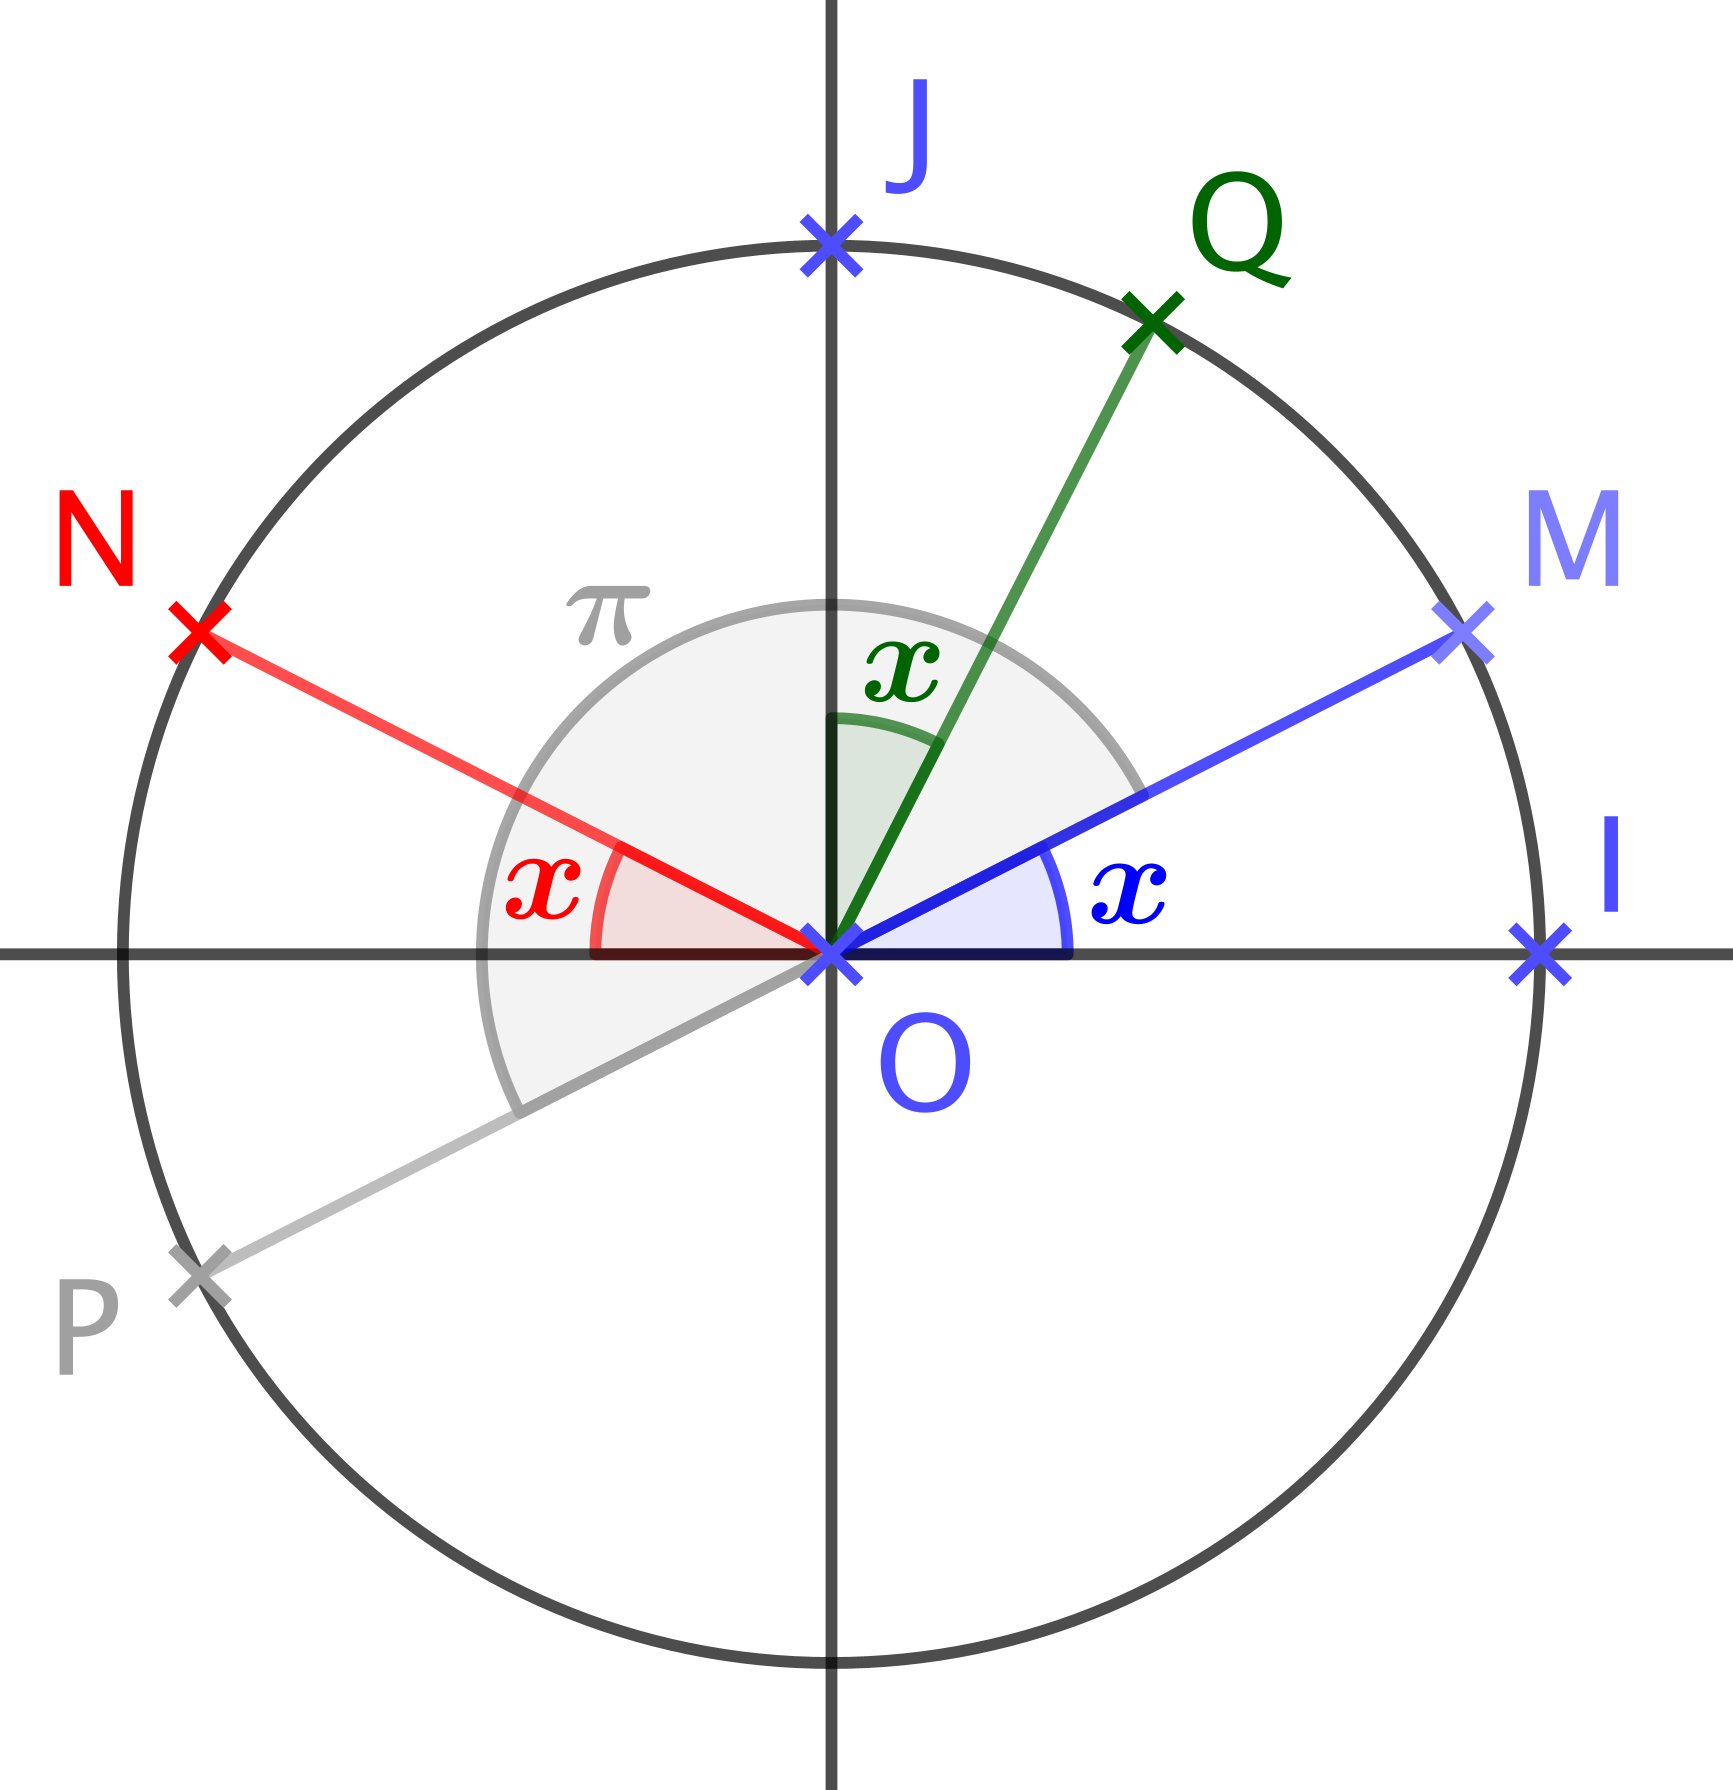
\includegraphics[scale = .7]{one-var-trig-formulas.png}
\end{center}

Via les points $M$, $N$, $P$ et $Q$, il est facile de fournir des arguments géométriques de symétrie justifiant que, sous la condition $x \in \intervalO{0}{\frac{\pi}{4}}$, nous avons:
%
\begin{multicols}{3}
\begin{itemize}[label=\small\textbullet]
	\item $\cos (\pi - x) = - \cos x$

	      \noindent
	      $\sin (\pi - x) = \sin x$ 

	\item $\cos (x + \pi) = - \cos x$

	      \noindent
	      $\sin (x + \pi) = - \sin x$

	\item $\cos \left( \frac{\pi}{2} - x \right) = \sin x$

	      \noindent
	      $\sin \left( \frac{\pi}{2} - x \right) = \cos x$ 
\end{itemize}
\end{multicols}


De nouveau, il serait bien de pouvoir passer, sans plus d'effort, à la validité des formules ci-dessus sur $\RR$ tout entier \emph{(considérer les autres cas n'est pas compliqué, mais c'est pénible)}.
%
Nous allons voir que cela est licite grâce au fait \ref{analytic-identity}, donné plus bas, qui est un peu technique, car il nécessite la notion de fonction analytique.


% ----------- %


\begin{preli} \label{XXX}
    Le rayon de convergence $R$ de la série entière complexe $\dsum_{k=0}^{\infty} a_k z^k$ est défini par la formule d'Hadamard
    $\displaystyle \frac{1}{R} = \limsup_{n \to \infty} \sqrt[n]{\abs{a_n}}$.
    %
    Ce nombre $R$ s'interprète comme suit.
    \begin{itemize}
        \item Si $R = 0$, la série ne converge que pour $z = 0$.

        \item Si $R = +\infty$, la série converge sur $\CC$, c'est-à-dire pour tout nombre complexe $z$.

        \item Si $0 < R < +\infty$, la série converge sur le disque ouvert $\CdiscO{0}{R}$, et elle diverge sur $\CC - \CdiscC{0}{R}$. Le comportement sur le cercle $\Ccircle{0}{R}$ se traite au cas par cas.
    \end{itemize}
\end{preli}


\begin{proof}
	TODO
	
	
	
	Considérons la série entière \( \sum a_n (x - x_0)^n \). Nous cherchons les valeurs de \( x \) pour lesquelles cette série converge absolument, c'est-à-dire lorsque la série \( \sum |a_n (x - x_0)^n| \) converge.

Un critère classique est le critère de d'Alembert :
\begin{equation}
    \limsup_{n \to \infty} \left| \frac{a_{n+1} (x - x_0)^{n+1}}{a_n (x - x_0)^n} \right| < 1.
\end{equation}
Cela donne :
\begin{equation}
    \limsup_{n \to \infty} \left| \frac{a_{n+1}}{a_n} \right| |x - x_0| < 1.
\end{equation}

On introduit la notion de \( \limsup \), qui mène à la condition générale :
\begin{equation}
    \limsup_{n \to \infty} |a_n|^{1/n} |x - x_0| < 1.
\end{equation}

Pour que cette inégalité soit satisfaite, il faut :
\begin{equation}
    |x - x_0| < \frac{1}{\limsup_{n \to \infty} |a_n|^{1/n}}.
\end{equation}

On définit alors le rayon de convergence \( R \) par :
\begin{equation}
    R = \frac{1}{\limsup_{n \to \infty} |a_n|^{1/n}}.
\end{equation}

Ainsi, la série converge absolument pour \( |x - x_0| < R \) et diverge pour \( |x - x_0| > R \).
\end{proof}


% ----------- %


\begin{preli} \label{XXX}
    Soit une série entière complexe $\dsum_{k=0}^{\infty} a_k z^k$ de rayon $R$ de convergence non nul.
    %
    La fonction $f: z \in \CdiscO{0}{R} \mapsto \dsum_{k=0}^{\infty} a_k z^k \in \CC$ est infiniment dérivable, au sens complexe, avec $\forall n \in \NN$, $\der[e]{f}{z}{n}(z) = \dsum_{k \geq n}^{\infty} \frac{n!}{k!} a_k z^{n - k}$.
\end{preli}


\begin{proof}
	TODO
\end{proof}


% ----------- %


\begin{defi}
    Soit $\Omega \subseteq \CC$ un ouvert non vide.
	%
	Une fonction $f: \Omega \rightarrow \CC$ est dite analytique en $z_0 \in \Omega$, 
	s'il existe
	une série entière $\dsum_{n = 0}^{+\infty} a_n z^n$
	de rayon de convergence $R > 0$,
	et
	un réel $r \in \intervalOC{0}{R}$ tels que dans le disque ouvert $\CdiscO{z_0}{r} \subseteq U$, on ait:
	$f(z) = \dsum_{n = 0}^{+\infty} a_n (z - z_0)^n$.

	\smallskip
	
	Si $f$ est analytique en tout complexe de $\Omega$,
	la fonction $f$ est dite analytique sur $\Omega$.
\end{defi}


% ----------- %


\begin{fact} \label{analytic-identity}
    Soit $\Omega \subseteq \CC$ un ouvert connexe non vide,
    et
    $f: \Omega \rightarrow \CC$ une fonction analytique.
    %
	Si $f$ s'annule sur un ouvert de $\Omega$, alors $f$ est identiquement nulle
	\emph{(c'est le théorème d'identité)}.  
\end{fact}


\begin{proof}
	TODO
\end{proof}


% ----------- %


\begin{fact} \label{power-series-vs-analytic}
    Soit $f: \Omega \rightarrow \CC$ où $\Omega \subseteq \CC$ est un ouvert non vide.
    %
    S'il existe
    $z_0 \in \CC$,
    et
    une série entière $\dsum_{n = 0}^{+\infty} a_n z^n$ de rayon de convergence infini
    telle que
	$\forall z \in \Omega$, $f(z) = \dsum_{n = 0}^{+\infty} a_n (z - z_0)^n$,
	alors
	$f$ est analytique sur $\Omega$. 
\end{fact}


\begin{proof}
	TODO
\end{proof}


Si nous revenons à nos identités trigonométriques, il suffit de savoir que les fonctions circulaires complexes sont analytiques sur $\CC$ tout entier, et de noter que le raisonnement géométrique au début de cette section fait clairement apparaître des zéros non isolés pour les fonctions analytiques sur $\CC$ suivantes.%
\footnote{
	Nous admettrons ces affirmations qui ne sont pas violentes à démontrer une fois que l'on a les bases de la théorie des fonctions analytiques.
}
%
\begin{itemize}[label=\small\textbullet]
	\item $f_1(z) = \cos (\pi - z) + \cos z$ 
	   et $f_2(z) = \sin (\pi - z) - \sin z$ 

	\smallskip
	\item $f_3(z) =\cos (z + \pi) + \cos z$ 
	   et $f_4(z) =\sin (z + \pi) + \sin z$

	\smallskip
	\item $f_5(z) =\cos \left( \frac{\pi}{2} - z \right) - \sin z$ 
	   et $f_6(z) =\sin \left( \frac{\pi}{2} - z \right) - \cos z$ 
\end{itemize}








%\newpage
%
%
%Que faire si nous avons des formules trigonométriques impliquant deux variables? Par exemple, le dessin suivant, par simple application des définitions géométriques du cosinus et du sinus, donne à la fois
%$\cos(\alpha + \beta) = \cos \alpha \cos \beta - \sin \alpha \sin \beta$
%et
%$\sin(\alpha + \beta) = \cos \alpha \sin \beta + \sin \alpha \cos \beta$
%pour
%$(\alpha ; \beta) \in \big( \RRsp \big)^2$ tel que $0 < \alpha + \beta < \frac{\pi}{2}$. 
%
%\begin{center}
%	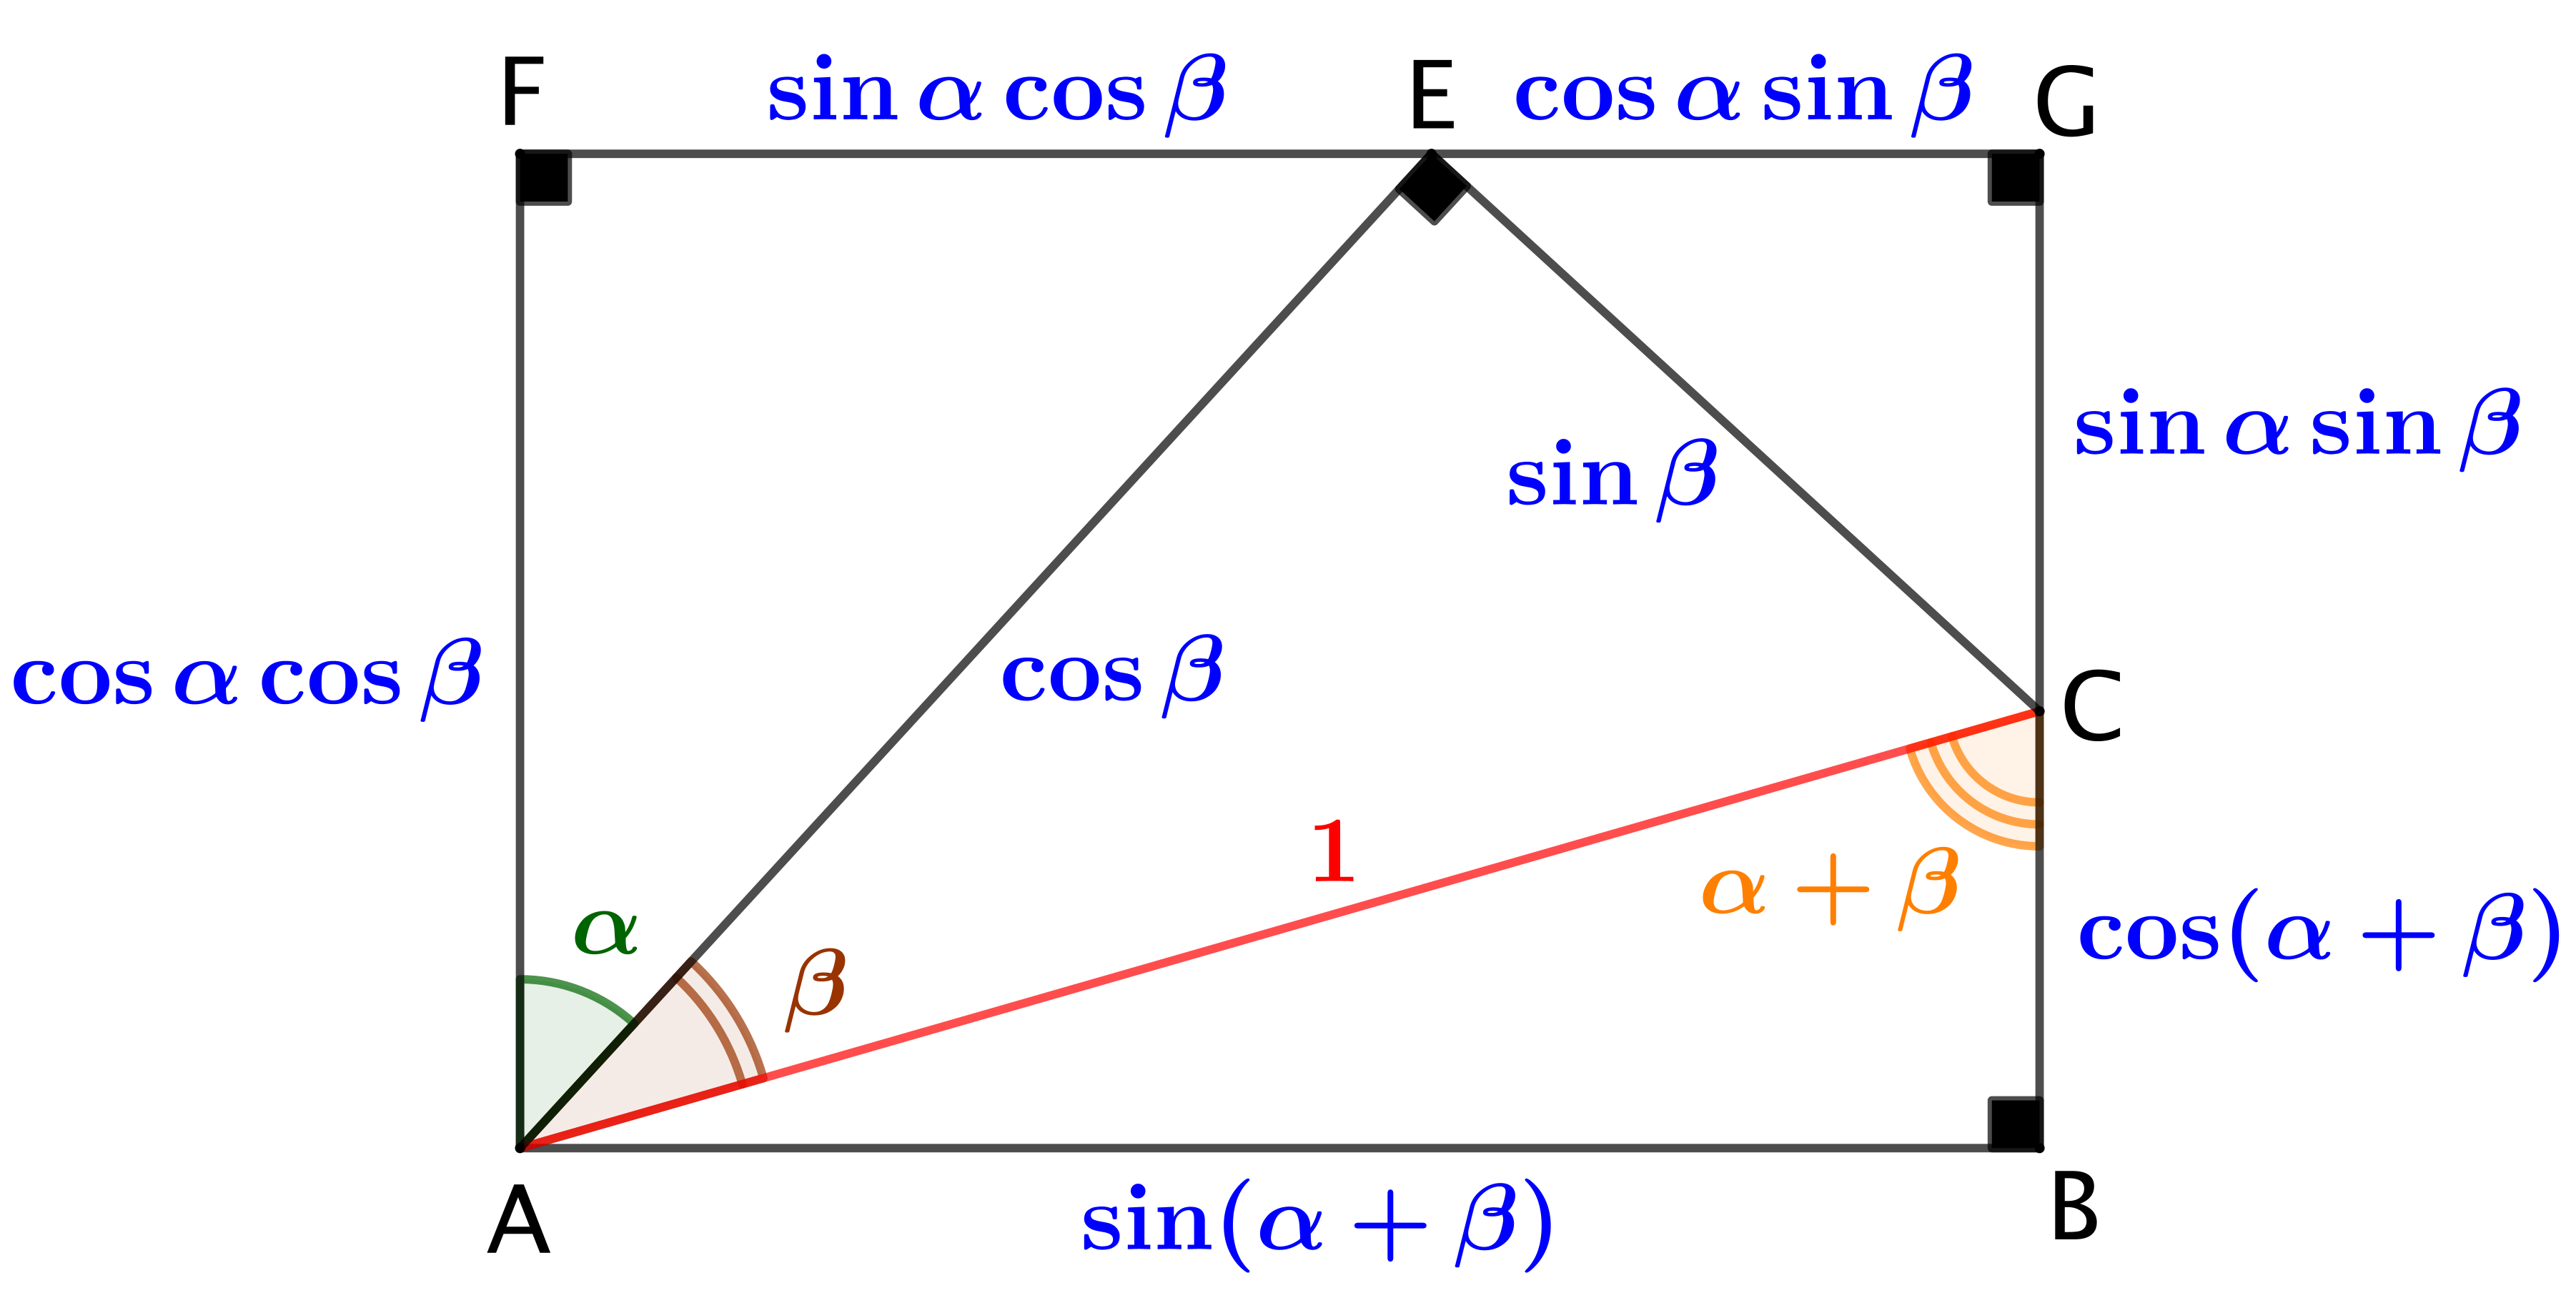
\includegraphics[scale=.7]{two-var-trig-formulas.png}
%\end{center}
%
%Le fait \ref{multi-analytic-identity} ci-dessous, qui généralise le fait \ref{analytic-identity}, implique la validité des formules trigonométriques précédentes sur $\RR^2$ tout entier en faisant les choix ci-après.
%Nous voilà sauvés!
%%
%\begin{itemize}[label=\small\textbullet]
%	\item $f_1(\alpha ; \beta) = \cos(\alpha + \beta) - \cos \alpha \cos \beta + \sin \alpha \sin \beta$
%
%	\item $f_2(\alpha ; \beta) = \sin(\alpha + \beta) - \cos \alpha \sin \beta - \sin \alpha \cos \beta$
%\end{itemize}
%
%
%
%
%
%
%\begin{defi}
%    Soient $n \in \NNs$, et $\Omega \subseteq \CC$ un ouvert non vide.
%	Une fonction $f: \Omega \rightarrow \CC$ est dite analytique en $z_0$, 
%	s'il existe
%	une série entière $\dsum_{n = 0}^{+\infty} a_n z^n$
%	de rayon de convergence $R > 0$,
%	et
%	un réel $r \in \intervalOC{0}{R}$ tels que dans le polydisque ouvert $\topodisc{z_0}{r} \subseteq U$, on ait:
%	$f(x) = \dsum_{XXX} a_n (x - z_0)^n$.
%	%
%	Si $f$ est analytique en tout complexe de $\Omega$, on dira que $f$ est analytique sur $\Omega$.
%\end{defi}
%
%
%
%\begin{fact} \label{multi-power-series-vs-analytic}
%    Soient $n \in \NNs$, et $f: \RR^n \rightarrow \RR$.
%    S'il existe une série entière $\dsum_{XXXX} a_n z^n$ de rayon de convergence infini
%    telle que
%	$\forall x \in \RR^n$, $f(x) = \dsum_{XXX} a_n z^n$,
%	alors
%	$f$ est analytique sur $\RR^n$. 
%\end{fact}
%
%
%\begin{proof}
%	TODO
%\end{proof}
%
%
%
%\begin{fact} \label{multi-analytic-identity}
%    Soient $n \in \NNs$, et $\Omega \subseteq \CC^n$ un ouvert connexe non vide,
%    et
%    $f: \Omega \rightarrow \CC$ une fonction analytique.
%    %
%	Si $f$ s'annule sur un ouvert de $\Omega$, alors $f$ est identiquement nulle
%	\emph{(c'est le théorème d'identité)}.  
%\end{fact}
%
%
%\begin{proof}
%	TODO
%\end{proof}